\section{Solution Algorithm}\label{sec:solution_algorithm}

A solution to the TRP is a collection of paths, one for each train, in the time-space graph $\STGraph$. The solution algorithm must be able to modify the forecast timetable in order to solve the conflicts, and to compute the new objective function. Key requirements for this algorithm, deriving from its real-time nature, are:
\begin{itemize}
	\item It must produce solutions of high quality in very short computational times (a few seconds). This is due to the fact that the algorithm is used on-line by dispatcher, who needs reasonable advice in few seconds, to guarantee the safety of operations in the network. For this reason, we focussed on a heuristic approach.
	\item If the algorithm is not able to find a conflict-free schedule, it has to give the dispatcher a schedule with the smallest possible number of remaining conflicts. This means that solving more conflicts needs to always have priority over other factors. In order to accomplish this, we established an implicit hierarchy through our objective function. A very high penalty is assigned to each unresolved conflict, so that a solution with fewer conflicts will always prevail on one which has more, while the ``standard'' objective function is used to decide the best one between two solutions with the same number of remaining conflicts. Therefore, the objective function presented in \eqref{eq:objf} is used as a part of the overall objective function: $\tilde{f}(\vec{x}) = P \cdot N_\textup{RC}(\vec{x}) + f(\vec{x})$, where $P$ is the large penalty to pay for each conflict, and $N_\textup{RC}$ gives the number of remaining conflicts in the solution.
	\item The algorithm should allow for a high degree of parallelisation, allowing to concurrently produce multiple rescheduled timetables that will be stored in a solution pool, from which the best one will be selected. This allows the algorithm to employ and evaluate different strategies in situations where none of them is clearly superior to the others, thereby focussing on different key aspects of the problem.
\end{itemize}

With these requirements in mind, we now give a general description of the algorithm which boradly falls into the category of iterated greedy algorithms (see, e.g., \citet{Ruiz20072033}). After an initialisation phase in which trains are ranked according to some criterion, the algorithm iterates among two main phases, until a termination condition is met. The two phases are:
\begin{enumerate}
	\item \textbf{Construction}: a new timetable is obtained by rescheduling the trains one by one, according to their ranking. \label{it:con}
	\item \textbf{Shaking}: the train ranking is perturbed following a set of rules. \label{it:sha}
\end{enumerate}
In our case the termination criterion is a hard time limit, with early termination if the solutions didn't improve over a certain number of iterations. The next subsections will describe each phase in detail. Furthermore, in order to speed up the computational time of the construction phase, we employed a sparsification of the graph $\STGraph$. This is a technique used to remove some edges and vertices from the time-space graph. Its use is justified by the fact that, by choosing a fine time discretisation, we might create a great number of edges, many of which can be removed without strongly impacting the quality of the train plans.

Notice that, for the algorithm initialisation, for the shaking phase, and for sparsification we propose several possible alternatives. Therefore, an instance of our algorithm is completely defined once we specify which initial sorting, shaking policy, and sparsification method is used. An extensive experimental testing of the proposed alternatives, described in \Cref{ssec:ptuning}, will help determining well-performing combinations of the algorithm's components.

\subsection{Initial sorting}

Since the algorithm constructs a schedule for one train at a time (Step \ref{it:con}), the order in which the trains are considered is clearly important, as trains scheduled later will be constrained by those scheduled earlier. Since there is no ``natural'' order of trains, we used various sorting criteria:
\begin{itemize}
	\item \textbf{Random}: the trains are randomly sorted.
	\item \textbf{Congestion}: the trains are sorted according to the number of conflicts in their forecast timetable, putting trains with more conflicts first. The rationale behind this choice is that a train that generates a lot of conflicts is harder to schedule, and therefore should be scheduled earler. Using the notation introduced earlier, if $\vec{x}^*$ is the assignment of variables corresponding with the forecast timetable, then we sort the trains by decreasing value of $N^\train_\textup{RC}(\vec{x}^*)$, where $N^\train_\textup{RC}(\vec{x}^*)$ is the number of conflicts in train $\train$'s schedule, and $N_\textup{RC}(\vec{x}^*) = \sum_{\train \in \Trains} N^\train_\textup{RC}(\vec{x}^*)$.
	\item \textbf{Length}: the trains are sorted according to the number of nodes in their original path in decreasing order. The longer the path, in fact, the higher the chances that a conflict will be present at some node. The trains are therefore sorted in decreasing order of the size of their set $\{ \arc \in \Arcs^\train \ : \ \vec{x}^* = 1 \}$.
	\item \textbf{Conflict time}: the trains are sorted according to the time instant of the earliest conflict in their forecast timetable. This is because an early conflict can impact the overall network status at a much later time. In other words, there is more freedom when fixing conflicts happening earlier, and we want to fully use this freedom.
	\item \textbf{Speed}: the trains with highest average speed are scheduled earlier. This strategy is based on the observation that faster trains have schedules that are more sensitive to variations. The average speed of a train $\train$ is given by:
  \begin{equation*}
    \frac{
      \sum_{\arc \in \STArcs^\train, \, \vec{x}^*_\arc = 1} \frac{\reslength(\arc)}{\etime(\arc) - \stime(\arc)}%
    }{%
      \left| \left\{ \arc \in \STArcs^\train \ : \ \etime(\arc) > \stime(\arc) \text{ and } \vec{x}^*_\arc = 1 \right\} \right|%
    }
  \end{equation*}
\end{itemize}
During a preliminary experimental phase, we noticed that using the sorting criteria in reverse order can sometimes lead to better results. For this reason we also considered the criteria \textbf{Reverse congestion} and \textbf{Reverse speed}.

\subsection{Construction}\label{ssec:construction}

Each train schedule is constructed by solving a shortest-path problem on the time-expanded graph $\STGraph$, where the starting node correspons to the current position of the train and the ending node corresponds to the train's desired position at the end of the time horizon.

Since trains run along fixed routes, with only a few possible detours, and since they have hard constraints on the time at which they can reach and leave certain resources, the graph $\STGraph$ can be pruned accordingly for each train. Once this is done, the shortest path is constructed with a custom label-setting algorithm. Given a partial path to a certain node $(\stnode, \timeinstant) \in \STNodes$, the corresponding label will be $L = ((\stnode', \timeinstant'), c)$ where the node $(\stnode', \timeinstant') \in \STNodes$ is the predecessor of $(\stnode, \timeinstant)$ in the partial path and $c \in \Rea$ is the cost of the partial path up to the current node.

Notice that, since trains are scheduled sequentially and the algorith is ran on a different time-space graph for each train, we cannot run into deadlocks. A deadlock will indeed correspond to an unresolved conflict (usually a capacity violation) and be accordingly heavily penalised in the objective function.

\begin{figure}
	\begin{center}
		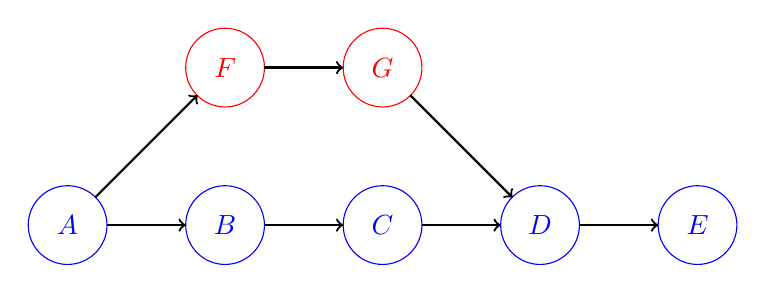
\begin{tikzpicture}
	\draw[blue] (0,0) circle[radius=0.5] node {$A$};
	\draw[blue] (2,0) circle[radius=0.5] node {$B$};
	\draw[blue] (4,0) circle[radius=0.5] node {$C$};
	\draw[blue] (6,0) circle[radius=0.5] node {$D$};
	\draw[blue] (8,0) circle[radius=0.5] node {$E$};
	\draw[red] (2,2) circle[radius=0.5] node {$F$};
	\draw[red] (4,2) circle[radius=0.5] node {$G$};
	
	\draw[->,thick] (0.5,0) -- (1.5,0);
	\draw[->,thick] (2.5,0) -- (3.5,0);
	\draw[->,thick] (4.5,0) -- (5.5,0);
	\draw[->,thick] (6.5,0) -- (7.5,0);
	\draw[->,thick] (0.35,0.35) -- (1.65,1.65);
	\draw[->,thick] (2.5,2) -- (3.5,2);
	\draw[->,thick] (4.35,1.65) -- (5.65,0.35);
\end{tikzpicture}
	\end{center}
	\caption{Topological order between nodes (resources) of a simple network.}\label{fig:toporder}
\end{figure}

We discuss now two main aspects of this algorithm: the order in which we extend the labels and how we update the cost component. Labels are extended greedily, i.e., starting from the one with the lowest cost component, but with one exception: a label related to a resource $\stnode$ will be extended only after all the labels related to resources $\stnode' \prec \stnode$ have already been extended (independently from the time interval), even if they have a higher cost. The relation $\prec$ is the topological order relation between nodes in the subgraph of $\NetGraph$ induced by the union of the path of the train $\trainpath_\train$ and all the detours in $\Detours_\train$. To better understand this rule, consider \Cref{fig:toporder}, which describes the topological setup of a network with a main corridor and a possible detour (via $F$ and $G$). Labels related to resource $D$, for example, will be extended only after all labels related to resources $A$, $B$, $C$, $F$ and $G$ have been extended, since $A \prec B \prec C \prec D$ and $A \prec F \prec G \prec D$.

The cost component is updated taking into account the various penalties included in the objective function. Some of these penalties, however, depend on the interaction between different trains. As an example, consider a connection between trains $\train_1$ and $\train_2$. If $\train_1$ is scheduled before $\train_2$, when we schedule $\train_1$ will just assume that the connection will be satisfied. If, when scheduling $\train_2$, we realise that the connection is broken, we will add the penalty on the objective function of $\train_2$.

Finally, we need to take special care in case of split/merge operations, as these require the presence of multiple trains on the same resource at the same time. When the partial path of an input train reaches one of these resources, we fix the schedule of the train up to that point, by choosing the lowest cost partial path (we first explore all non-dominated partial paths up to the synchronisation point). We proceed with the construction of the schedule for the output trains, only once all the schedules of the input trains have been fixed up to the considered resource.

\subsection{Shaking}

In the shaking phase we perturb the ordering of the trains (the \emph{dispatching sequence}) with the aim of finding an ordering which leads, through a new construction phase, to an improving solution. We present two alternative policies, inspired to two well-known metaheuristic algorithms: Reduced Variable Neighbourhood Search (RVNS) and Tabu Search (TS). As mentioned in the beginning of this section, these two alternative policies are experimentally evaluated in \Cref{sec:computational_results}.

The RVNS (see, for example, \citet{Hansen2010}) explores the solution space of the problem by employing a sequence of neighbourhood structures $\nbstruct_1, \ldots, \nbstruct_{K}$. A neighbourhood structure defines a way to describe the neighbourhood of any solution $x$ in the solution space.

Starting from a solution $x$, RVNS generates a new random solution $x' \in \nbstruct_1(x)$. If the new solution is not better than the previous one, it goes on to the second neighbourhood structure and generates a random $x' \in \nbstruct_2(x)$. The procedure continues until either we run out of neighbourhood structures or the new solution $x'$ is better than the current one $x$. In the first case, the algorithm terminates; in the second case, the algorithm is restarted using $x'$ as initial solution and going back to using $\nbstruct_1$.

The neighbourhood structures are typically such that
\begin{equation}
	\nbstruct_1(x) \subseteq \nbstruct_2(x) \subseteq \ldots \subseteq \nbstruct_K(x) \label{eq:nbstruct}
\end{equation}
for all solutions $x$. This means that while no improving solution is found, the search space around $x$ is enlarged.

In our case, the neighbourhood structure $\nbstruct_k(x)$ consist in considering all dispatching orders that can be obtained from $x$ by performing at most $k$ swaps. From this definition, it follows immediately that \eqref{eq:nbstruct} is satisfied. The trains to be moved in the new dispatching order are selected at random with a roulette wheel selection procedure where the probability associated to each train is proportional to its contribution to the objective value. The number of positions each train is moved up is again chosen at random, according to a uniform distribution in $[\minmove, \maxmove]$.

The second policy is inspired to Tabu Search. Starting from a dispatching sequence, we produce a new one analogously to what done with the RVNS policy. We will place in our tabu list the precedence relations between the moved trains. For example, if we transform the sequence $x = (A,B,C,D)$ into $x' = (A,D,B,C)$, we will store the precedence relations $(D,B)$ and $(D,C)$. While these are in the tabu list, the relative order of trains $D,B$ and $D,C$ will not be inverted. If, at the next iteration, train $B$ will be selected to be moved up, then train $D$ will have to move together with $B$, so not to invert the relation $(D,B)$; the new dispatching sequence will then be $(D,B,A,C)$.

The number of iterations each precedence move is stored in the tabu list depends on three factors:
\begin{enumerate}
	\item The change in the part of the objective function relative to the moved train;
	\item The change in the overall objective function;
	\item Whether the new solution improved the incumbent solution.
\end{enumerate}

\subsection{Sparsification}\label{ssec:sparsification}

As previously mentioned, the sparsification of the graph $\STGraph$ is used to remove some edges and vertices from the time-space graph, to speed up the computation of shortest paths by the labelling algorithm. Its use is justified by the fact that, by choosing a fine time discretisation, we might create a great number of edges, many of which can be removed without strongly impacting the quality of the train plans.

As an example, consider a segment of track 5km long and a train that, at full speed, would travel on this segment at 100km/h. The running time of this train will be of 3 minutes. If we choose time intervals to represent 1 second, that would be 180 time instants. If the entry point is $\stnode^\textup{L}$ and the exit point is $\stnode^\textup{R}$, when we consider an entry time of $\timeinstant$, we would create all the arcs
\begin{equation*}
	\left( \left( \stnode^\textup{L}, t \right), \left( \stnode^\textup{R}, t + 180 \right) \right),
	\left( \left( \stnode^\textup{L}, t \right), \left( \stnode^\textup{R}, t + 181 \right) \right),
	\left( \left( \stnode^\textup{L}, t \right), \left( \stnode^\textup{R}, t + 182 \right) \right), \ldots
\end{equation*}
up to the end of the time horizon. This level of accuracy is clearly not needed in this situation: a train that took 181 time instants rather than 180 to travel along that segment, would go at a speed of 99.45km/h which is indistinguishable from 100km/h for any practical purpose. So, even if removing some edge from the graph would --- in principle --- cause the algorithm to miss some feasible train plan, if these edges are properly selected, we can easily reduce the probability to miss a train plan that would produce a considerable improvement.

Here we propose four main strategies for graph sparsification. Let $\node$ be a node in the network, $\train$ the train under consideration and $\mintraveltime_{\train,\node}$ the minimum travel time of $\train$ along $\node$. Furthermore, let $\timeinstant$ be the entry time of the train at the node and $\timeinstant'$ the first feasible exit time, taking into account both the minimum travel time and the other constraints such as the minimum and maximum out-times $\minouttime_{\train,\node}$ and $\maxouttime_{\train,\node}$. The strategies we used are the following:
\begin{description}
	\item[Fixed step] We only consider departure times starting at $\timeinstant'$ and then keeping a time instant in every $\timestep$. The set of possible departure times will be
	\begin{equation*}
		\left\{ \left. \timeinstant' + k \cdot \timestep \ \right| \ k = 0, 1, \ldots \right\}
	\end{equation*}
	\item[Fixed step with threshold] The previous strategy can be improved by specifying a threshold $\timethreshold$ and keeping all departure times between $\timeinstant'$ and $\timeinstant' + \timethreshold$. In this way we keep those arcs that are close to $\timeinstant'$ and therefore correspond to a minimal delay of the train.
	\item[Linear] This case is similar to the fixed step sparsification, but the step $\timestep$ is adjusted to be inversely proportional to $\mintraveltime_{\train,\node}$. The set of possible departure times is
	\begin{equation*}
		\left\{ \left. \timeinstant' + k \cdot \max \left(1, \frac{\mintraveltime_{\train,\node}}{\timestep} \right) \ \right| \ k = 0, 1, \ldots \right\}
	\end{equation*}
	\item[Progressive] With this strategy we allow a higher density for time instants close to $t'$, while we retain fewer arcs as long as we move away from that time instant. The idea behind this criterion is that good train plans are characterised by train schedules that are delayed as little as possible. The set of possible departure times is $\left\{ \timeinstant'_k \right\}$ where $\timeinstant'_0 = t'$ and
	\begin{equation*}
		\timeinstant'_k = \timeinstant'_{k-1} + 1 + \left\lfloor \frac{\timeinstant'_{k-1} - t}{\timestep} \right\rfloor
	\end{equation*}
\end{description}
In our testing we used $s \in \{ 2, 3, 5 \}$ and $\tau \in \{ 5, 10, 15 \}$, leading to a total of 19 combinations, including the case when sparsification is disabled. \Cref{fig:no_spars,fig:fixed_spars,fig:threshold_spars,fig:progressive_spars} give a graphical representation of the sparsification methods for a segment $\node$ with endpoints $\stnode_1^\textup{L}$ and $\stnode_2^\textup{R}$ and a minimum travel time $\mintraveltime_{\train,\node} = 2$.

\begin{figure}
  \centering
  \begin{subfigure}[ht]{\textwidth}
    \centering
    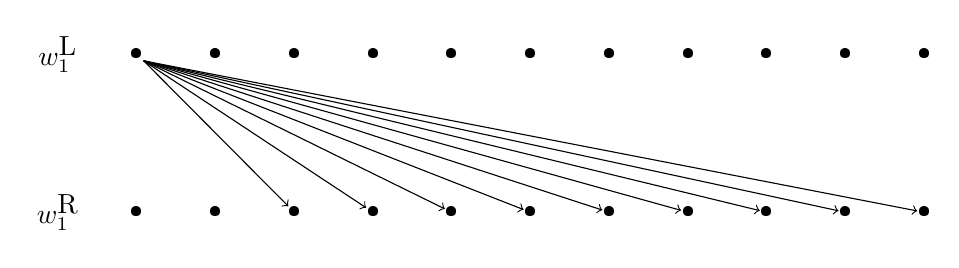
\begin{tikzpicture}
      \node at (-1,2) {$w_1^\textup{L}$};
      \node at (-1,0) {$w_1^\textup{R}$};
      \foreach \x in {0,...,10}
        \foreach \y in {0,...,1}
          \node[inner sep=0,outer sep=0] (n\y\x) at (\x,2*\y) {\textbullet};
      \foreach \x in {2,...,10}
        \draw[->] (n10.south east) -- (n0\x);
    \end{tikzpicture}
    \caption{No sparsification.}\label{fig:no_spars}
  \end{subfigure}
  \par\bigskip\bigskip
  \begin{subfigure}[ht]{\textwidth}
    \centering
    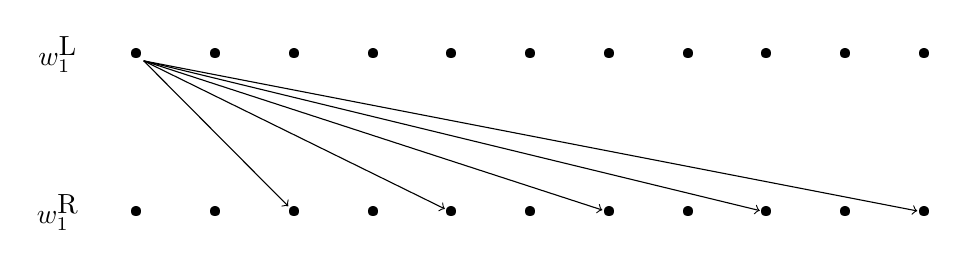
\begin{tikzpicture}
      \node at (-1,2) {$w_1^\textup{L}$};
      \node at (-1,0) {$w_1^\textup{R}$};
      \foreach \x in {0,...,10}
        \foreach \y in {0,...,1}
          \node[inner sep=0,outer sep=0] (n\y\x) at (\x,2*\y) {\textbullet};
      \foreach \x in {1,...,5}
        {\pgfmathtruncatemacro{\doublex}{\x * 2} \draw[->] (n10.south east) -- (n0\doublex);}
    \end{tikzpicture}
    \caption{Fixed step sparsification with $s = 2$.}\label{fig:fixed_spars}
  \end{subfigure}
  \par\bigskip\bigskip
  \begin{subfigure}[ht]{\textwidth}
    \centering
    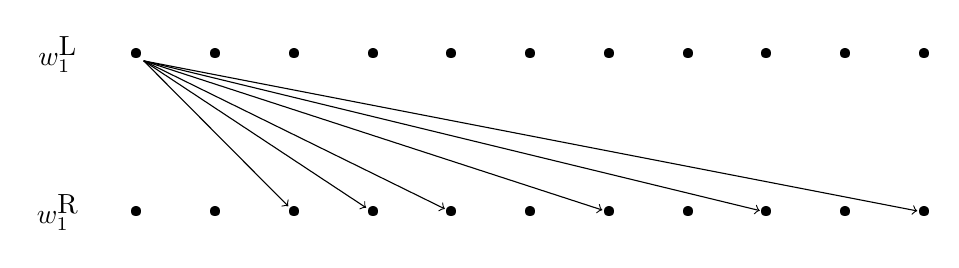
\begin{tikzpicture}
      \node at (-1,2) {$w_1^\textup{L}$};
      \node at (-1,0) {$w_1^\textup{R}$};
      \foreach \x in {0,...,10}
        \foreach \y in {0,...,1}
          \node[inner sep=0,outer sep=0] (n\y\x) at (\x,2*\y) {\textbullet};
      \foreach \x in {1,...,5}
        {\pgfmathtruncatemacro{\doublex}{\x * 2} \draw[->] (n10.south east) -- (n0\doublex);}
      \draw[->] (n10.south east) -- (n03);
    \end{tikzpicture}
    \caption{Fixed step sparsification with $s = 2$ and threshold $\tau = 3$.}\label{fig:threshold_spars}
  \end{subfigure}
  \par\bigskip\bigskip
  \begin{subfigure}[ht]{\textwidth}
    \centering
    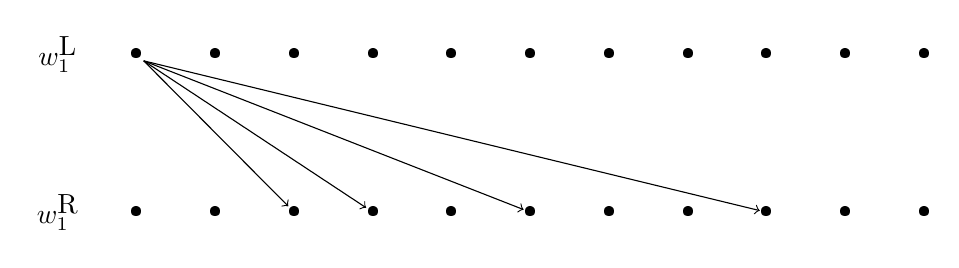
\begin{tikzpicture}
      \node at (-1,2) {$w_1^\textup{L}$};
      \node at (-1,0) {$w_1^\textup{R}$};
      \foreach \x in {0,...,10}
        \foreach \y in {0,...,1}
          \node[inner sep=0,outer sep=0] (n\y\x) at (\x,2*\y) {\textbullet};
      \draw[->] (n10.south east) -- (n02);
      \draw[->] (n10.south east) -- (n03);
      \draw[->] (n10.south east) -- (n05);
      \draw[->] (n10.south east) -- (n08);
    \end{tikzpicture}
    \caption{Progressive sparsification.}\label{fig:progressive_spars}
  \end{subfigure}
  \caption{Graphical representation of various graph sparsification techniques on the time-space graph.}\label{fig:spars}
\end{figure}
